\newpage
\subsection{Working with multple MOSL projects}
\texHeader
\label{sec:multiMOSL}

% Eclipse import instructions; all unconfirmed.

\begin{itemize}

\item[$\blacktriangleright$] With your source metamodel, \texttt{LeitnersLearningBox} prepared in the Eclipse workspace, right-click on \texttt{MyWorkingSet}
and select \texttt{Import\ldots} from the context menu (Fig.~\ref{fig:eclipseContextImport}).

\begin{figure}[htbp]
\begin{center}
  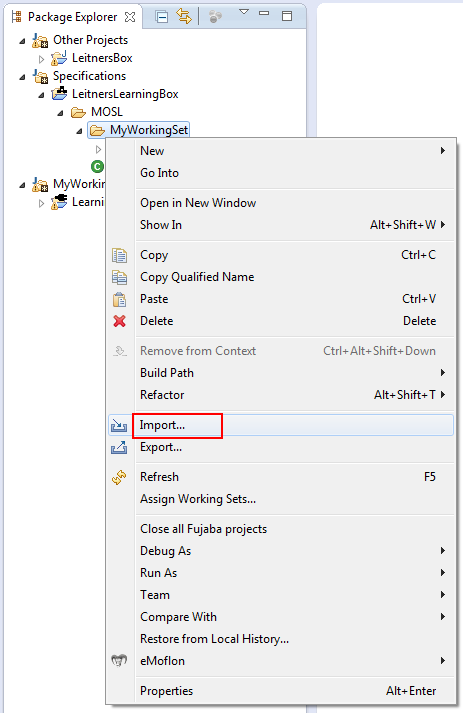
\includegraphics[width=0.6\textwidth]{eclipse_contextImport}
  \caption{caption}
  \label{fig:eclipseContextImport}
\end{center}
\end{figure}

\item[$\blacktriangleright$] In the first import dialogue, set your import source by navigating to ``General/File System.'' This is the appproate choice since
we want to import the entire directory structure of the target metamodel. Continue by pressing \texttt{Next >}.

\item[$\blacktriangleright$] Press \texttt{Browse\ldots} (Fig.~\ref{fig:importFileSys}) and navigate to the folder where you extracted the contents of the
\texttt{Part4.zip} file which included this document. Select \texttt{DictionaryLanguage} from the heirarchy, and affirm with \texttt{OK}.

\item[$\blacktriangleright$] Press \texttt{Select All} to ensure you're importing all the necessary MOSL files for your TGG target \texttt{DictionaryLanguage}
metamodel. Affirm and close the dialogue by pressing \texttt{Finish}.

\begin{figure}[htbp]
\begin{center}
  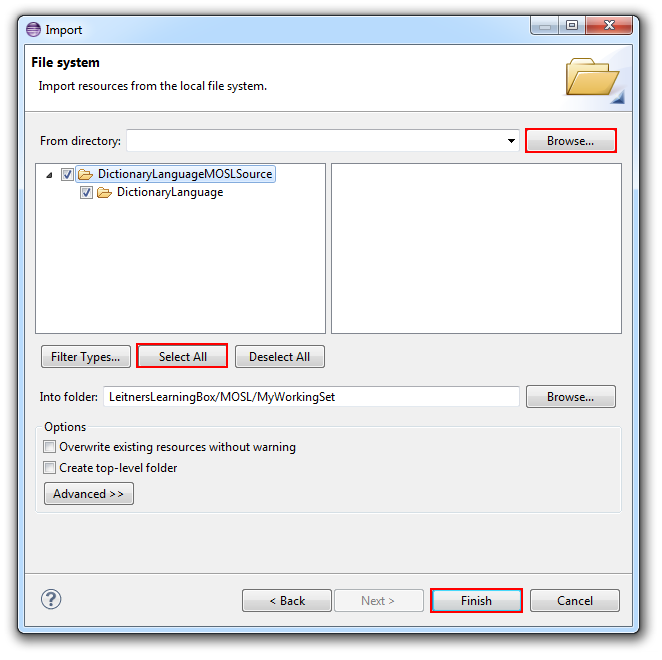
\includegraphics[width=0.8\textwidth]{eclipse_importDialogue}
  \caption{caption}
  \label{fig:importFileSys}
\end{center}
\end{figure}

\item[$\blacktriangleright$] Navigate to ``Build (Without Cleaning)'' on the toolbar to build both metamodels. Confirm with
Fig.~\ref{fig:bothmetamodelstructures} that your MOSL directory is now populated with both metamodels, and notice that a second \texttt{Dictionary\-Language}
folder appeared under the same node as the \texttt{LearningBoxLanguage} repository project. If you expand this folder, you'll be able to see that it contains
all the generated code for the imported metamodel.

\begin{figure}[htbp]
\begin{center}
  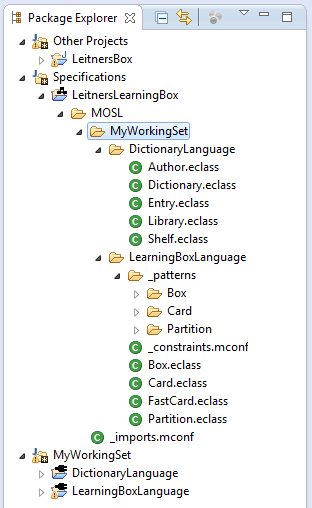
\includegraphics[width=0.5\textwidth]{eclipse_metamodelStructures}
  \caption{caption}
  \label{fig:bothmetamodelstructures}
\end{center}
\end{figure}

\item[$\blacktriangleright$] You're now ready to start using your metamodels in a TGG transformation! If you've just joined us and are interested in the eMoflon
project structure, or curious as to how Java code is generated, we invite you to read Section 4.2 from Part I. Otherwise, continue to the next section to begin
building your TGG Schema. !Confirm it was imported into \texttt{MyWorkingSet}, and not just \texttt{MOSL}. That is wrong / different reference location.

\end{itemize}
